\section{Introduction}\label{sec:intro}

Search and rescue robots often need to find source of a signal like radio-active material, heat signature or gas leak. 
This problem is known as stochastic source seeking.
To plan an optimal exploration trajectory, many researchers~\cite{atanasov2014StochasticSourceSeeking} have suggested using 
information gain metrics like Mutual Information.
However, in partially observable environments computing information gain of 
a trajectory becomes challenging if parts of map are unknown. 
We address this problem by predicting unknown maps as an image inpainting problem.

Stochastic source seeking has been typically addressed in fully
   observable environments, with a single target~\cite{atanasov2014StochasticSourceSeeking}.
   On the other hand, exploration in partially observable
   environment~\cite{choudhury2017adaptive} has dealt
   with exploration without a source seeking objective.
We show how existing approaches that depend upon fully observable state do
not generalize to all kind of maps and obstacles. 

%Specifically, we consider a U-maze (Fig~\ref{fig:c-maze}), which has local optima with respect to greedy source seeking.
The work closest to our approach is Shreshta~et~al.~\cite{shreshta2019icra}.
However, they attempt to predict large regions in the map which are unlikely to generalize to new maps.
Moreover, Shreshta~et~al.~\cite{shreshta2019icra} use a flood fill over the
predicted map to estimate the information gain for each action. 
Flood filling can be brittle and lead to misleading information gains with even small holes in the walls of the map.
Instead, we predict only the occupancy of the to be filled in the next few laser scans and the possible information gained next few steps.
Further, Shreshta~et~al.~\cite{shreshta2019icra} evaluate there algorithm on simple map exploration task. 
To the best of our knowledge, map prediction has not been yet applied to source seeking.

We extend the source seeking approaches to partially observable environments
while building the map of the environment. We learn priors over the maps of
indoor buildings and predict unknown parts of the maps using Generative
Adversarial Networks~\cite{goodfellow2014GAN}, specifically
DeepFill~\cite{yu2018DeepFill}. With the map-predictive abilities, we apply
standard techniques used for Mutual Information maximization when map is known.
We show how our approach overcomes the challenges introduced by the
\emph{C-Maze} (Fig~\ref{fig:c-maze}).

%
\begin{figure}%
  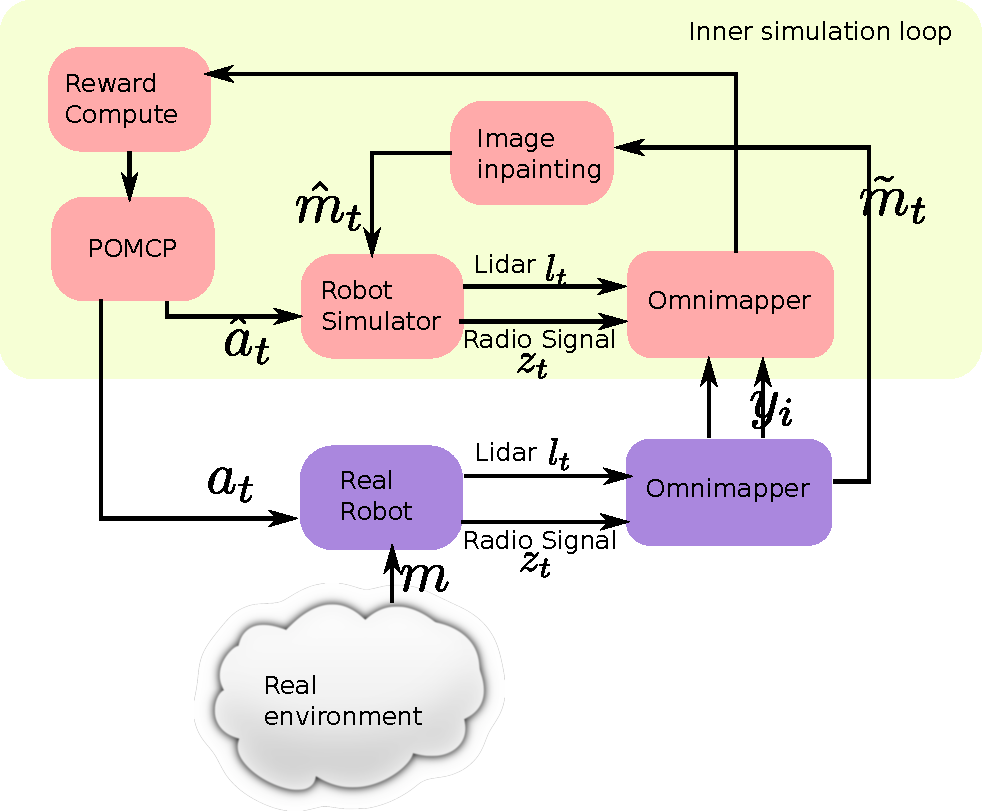
\includegraphics[width=\columnwidth]{files/media/overall-architecture.pdf}
  \caption{Overall architecture}%
  \label{fig:architecture}%
\end{figure}%
% 
